\documentclass[a4paper,11pt]{article}
\usepackage[T1]{fontenc}
\usepackage[utf8]{inputenc}
\usepackage[english]{babel}
\usepackage{amsmath,amssymb,mathtools}
\usepackage[margin=2.2cm]{geometry}
\usepackage{tikz}
\usepackage[most]{tcolorbox}
\setlength{\parindent}{0pt}
\setlength{\parskip}{5pt}
\providecommand{\explainmode}{0}
\newif\ifexplain
\ifnum\explainmode=1 \explaintrue\fi
\newtcolorbox{erklbox}{colback=blue!4,colframe=blue!40,breakable,boxrule=.5pt,title=Erklärung}
\newcommand{\explain}[1]{\ifexplain\begin{erklbox}#1\end{erklbox}\fi}
\newcommand{\explainfig}[1]{\ifexplain\begin{center}#1\end{center}\fi}
\newcommand{\why}[1]{\text{\small #1}}
\newcommand{\angabe}[1]{\textit{#1}\par}
\newcommand{\aufgabe}[1]{\section*{Exercise #1}}
\newcommand{\teil}[1]{\subsection*{(#1)}}
\newcommand{\at}[1]{\texttt{#1}}
\begin{document}
\begin{center}{\Large Homework sheet 1}\\Logic Programming (621.315), Winter semester 2026\\Raphael Bleier\\Correction: 28 October 2026\end{center}
\explain{Ein Atom ist hier eine einzelne Aussage, etwa $\at{bird(tweety)}$. Ein Modell erfüllt alle Regeln, muss aber nicht die kleinste begründbare Menge sein. Ein Answer Set ist die kleinste abgeschlossene Menge seines eigenen Redukts. Default-Negation \texttt{not a} prüft, ob $a$ im Kandidaten fehlt; sie ist keine zusätzliche Aussage $\neg a$. Wir verwenden die Begriffe und die Notation $\operatorname{Cn}(P)$ aus den Kursnotizen zu positiven und normalen Programmen.}
\aufgabe{1.1}
\angabe{Determine the answer set of the following positive logic programs.}
\teil{a}
Rule numbers refer to the following order (one rule ends at each period).
\begin{small}
\begin{verbatim}
a :- b, d.
a :- c, e.
b :- d, m.
b :- e, f.
c :- d, e.
d.
e :- d.
f :- b, c.
g :- d, f.
g :- e, h.
h :- c, k.
k :- a, e.
\end{verbatim}
\end{small}
\explain{Das Programm enthält keine Default-Negation. Wir beginnen bei der leeren Menge und wenden nur Regeln an, deren Körper bereits erfüllt ist. Fakten starten die Herleitung. Eine positive Schleife ohne diesen Start liefert dagegen keine Atome.}
\[
M_0=\varnothing
\]
\begin{align*}
M_{1} &= M_{0}\cup \{\at{d}\} && \why{fact, rule 6}
\end{align*}
\explain{Diese Regel hat keinen Körper. Ihr Kopf $\at{d}$ ist damit ein Fakt und muss in die Menge.}
\begin{align*}
M_{2} &= M_{1}\cup \{\at{e}\} && \why{rule 7}
\end{align*}
\explain{Für $\at{e}$ brauchen wir $\at{d}$. Weil diese Voraussetzungen bereits hergeleitet sind, dürfen wir den Regelkopf jetzt aufnehmen und alle bisherigen Atome behalten; bei einer fehlenden Voraussetzung würde diese Regel dagegen noch nichts beitragen.}
\begin{align*}
M_{3} &= M_{2}\cup \{\at{c}\} && \why{rule 5}
\end{align*}
\explain{Für $\at{c}$ brauchen wir $\at{d}$ und $\at{e}$. Weil diese Voraussetzungen bereits hergeleitet sind, dürfen wir den Regelkopf jetzt aufnehmen und alle bisherigen Atome behalten; bei einer fehlenden Voraussetzung würde diese Regel dagegen noch nichts beitragen.}
\begin{align*}
M_{4} &= M_{3}\cup \{\at{a}\} && \why{rule 2}
\end{align*}
\explain{Für $\at{a}$ brauchen wir $\at{c}$ und $\at{e}$. Weil diese Voraussetzungen bereits hergeleitet sind, dürfen wir den Regelkopf jetzt aufnehmen und alle bisherigen Atome behalten; bei einer fehlenden Voraussetzung würde diese Regel dagegen noch nichts beitragen.}
\begin{align*}
M_{5} &= M_{4}\cup \{\at{k}\} && \why{rule 12}
\end{align*}
\explain{Für $\at{k}$ brauchen wir $\at{a}$ und $\at{e}$. Weil diese Voraussetzungen bereits hergeleitet sind, dürfen wir den Regelkopf jetzt aufnehmen und alle bisherigen Atome behalten; bei einer fehlenden Voraussetzung würde diese Regel dagegen noch nichts beitragen.}
\begin{align*}
M_{6} &= M_{5}\cup \{\at{h}\} && \why{rule 11}
\end{align*}
\explain{Für $\at{h}$ brauchen wir $\at{c}$ und $\at{k}$. Weil diese Voraussetzungen bereits hergeleitet sind, dürfen wir den Regelkopf jetzt aufnehmen und alle bisherigen Atome behalten; bei einer fehlenden Voraussetzung würde diese Regel dagegen noch nichts beitragen.}
\begin{align*}
M_{7} &= M_{6}\cup \{\at{g}\} && \why{rule 10}
\end{align*}
\explain{Für $\at{g}$ brauchen wir $\at{e}$ und $\at{h}$. Weil diese Voraussetzungen bereits hergeleitet sind, dürfen wir den Regelkopf jetzt aufnehmen und alle bisherigen Atome behalten; bei einer fehlenden Voraussetzung würde diese Regel dagegen noch nichts beitragen.}
No rule has a true body and a head outside $M_{7}$; hence this is the least fixed point.
\[
\operatorname{Cn}(R)=\{\at{a},\;\at{c},\;\at{d},\;\at{e},\;\at{g},\;\at{h},\;\at{k}\}
\]
The atom $m$ has no head rule. The remaining support for $b,f$ is a positive cycle with no initial fact. Neither is derived.
\explainfig{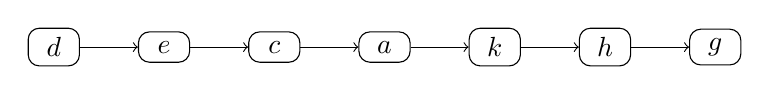
\begin{tikzpicture}[every node/.style={draw,rounded corners,minimum width=.65cm}]\node (d) at (0,0) {$d$};\node (e) at (1.4,0) {$e$};\node (c) at (2.8,0) {$c$};\node (a) at (4.2,0) {$a$};\node (k) at (5.6,0) {$k$};\node (h) at (7,0) {$h$};\node (g) at (8.4,0) {$g$};\draw[->] (d)--(e);\draw[->] (e)--(c);\draw[->] (c)--(a);\draw[->] (a)--(k);\draw[->] (k)--(h);\draw[->] (h)--(g);\end{tikzpicture}}
\explain{Die Grafik zeigt die Reihenfolge der neuen Atome, nicht den vollständigen Regelkörper. Frühere Voraussetzungen bleiben erhalten: Für $c$ brauchen wir etwa $d$ und $e$, für $a$ dann $c$ und $e$. Die genaue Begründung steht deshalb bei jedem einzelnen Schritt.}
\[
\boxed{X=\{\at{a},\;\at{c},\;\at{d},\;\at{e},\;\at{g},\;\at{h},\;\at{k}\}}
\]
\explain{Die Probe besteht aus zwei Teilen: Jede aufgenommene Aussage hat oben eine passende Regel. Am Ende kann keine Regel ein weiteres Atom hinzufügen. Damit ist die Menge ein Modell und zugleich das kleinste Modell.}
\teil{b}
Rule numbers refer to the following order (one rule ends at each period).
\begin{small}
\begin{verbatim}
conn(amsterdam,brussels).
conn(brussels,cologne).
conn(cologne,amsterdam).
tour(amsterdam,cologne) :- conn(amsterdam,brussels),
    conn(brussels,cologne).
tour(brussels,amsterdam) :- conn(brussels,cologne),
    conn(cologne,amsterdam).
tour(cologne,brussels) :- conn(amsterdam,brussels),
    conn(cologne,amsterdam).
finish(cologne) :- conn(amsterdam,amsterdam), tour(amsterdam,cologne).
finish(amsterdam) :- conn(brussels,amsterdam), tour(brussels,amsterdam).
finish(brussels) :- conn(cologne,amsterdam), tour(cologne,brussels).
\end{verbatim}
\end{small}
\explain{Das Programm enthält keine Default-Negation. Wir beginnen bei der leeren Menge und wenden nur Regeln an, deren Körper bereits erfüllt ist. Fakten starten die Herleitung. Eine positive Schleife ohne diesen Start liefert dagegen keine Atome.}
\[
M_0=\varnothing
\]
\begin{align*}
M_{1} &= M_{0}\cup \{\at{conn(amsterdam,brussels)}\} && \why{fact, rule 1}
\end{align*}
\explain{Diese Regel hat keinen Körper. Ihr Kopf $\at{conn(amsterdam,brussels)}$ ist damit ein Fakt und muss in die Menge.}
\begin{align*}
M_{2} &= M_{1}\cup \{\at{conn(brussels,cologne)}\} && \why{fact, rule 2}
\end{align*}
\explain{Diese Regel hat keinen Körper. Ihr Kopf $\at{conn(brussels,cologne)}$ ist damit ein Fakt und muss in die Menge.}
\begin{align*}
M_{3} &= M_{2}\cup \{\at{conn(cologne,amsterdam)}\} && \why{fact, rule 3}
\end{align*}
\explain{Diese Regel hat keinen Körper. Ihr Kopf $\at{conn(cologne,amsterdam)}$ ist damit ein Fakt und muss in die Menge.}
\begin{align*}
M_{4} &= M_{3}\cup \{\at{tour(amsterdam,cologne)}\} && \why{rule 4}
\end{align*}
\explain{Für $\at{tour(amsterdam,cologne)}$ brauchen wir $\at{conn(amsterdam,brussels)}$ und $\at{conn(brussels,cologne)}$. Weil diese Voraussetzungen bereits hergeleitet sind, dürfen wir den Regelkopf jetzt aufnehmen und alle bisherigen Atome behalten; bei einer fehlenden Voraussetzung würde diese Regel dagegen noch nichts beitragen.}
\begin{align*}
M_{5} &= M_{4}\cup \{\at{tour(brussels,amsterdam)}\} && \why{rule 5}
\end{align*}
\explain{Für $\at{tour(brussels,amsterdam)}$ brauchen wir $\at{conn(brussels,cologne)}$ und $\at{conn(cologne,amsterdam)}$. Weil diese Voraussetzungen bereits hergeleitet sind, dürfen wir den Regelkopf jetzt aufnehmen und alle bisherigen Atome behalten; bei einer fehlenden Voraussetzung würde diese Regel dagegen noch nichts beitragen.}
\begin{align*}
M_{6} &= M_{5}\cup \{\at{tour(cologne,brussels)}\} && \why{rule 6}
\end{align*}
\explain{Für $\at{tour(cologne,brussels)}$ brauchen wir $\at{conn(amsterdam,brussels)}$ und $\at{conn(cologne,amsterdam)}$. Weil diese Voraussetzungen bereits hergeleitet sind, dürfen wir den Regelkopf jetzt aufnehmen und alle bisherigen Atome behalten; bei einer fehlenden Voraussetzung würde diese Regel dagegen noch nichts beitragen.}
\begin{align*}
M_{7} &= M_{6}\cup \{\at{finish(brussels)}\} && \why{rule 9}
\end{align*}
\explain{Für $\at{finish(brussels)}$ brauchen wir $\at{conn(cologne,amsterdam)}$ und $\at{tour(cologne,brussels)}$. Weil diese Voraussetzungen bereits hergeleitet sind, dürfen wir den Regelkopf jetzt aufnehmen und alle bisherigen Atome behalten; bei einer fehlenden Voraussetzung würde diese Regel dagegen noch nichts beitragen.}
No rule has a true body and a head outside $M_{7}$; hence this is the least fixed point.
\[
\operatorname{Cn}(R)=\left\{\begin{gathered}\at{conn(amsterdam,brussels)},\;\at{conn(brussels,cologne)},\\\at{conn(cologne,amsterdam)},\;\at{finish(brussels)},\\\at{tour(amsterdam,cologne)},\\\at{tour(brussels,amsterdam)},\;\at{tour(cologne,brussels)}\end{gathered}\right\}
\]
The bodies for $\at{finish(cologne)}$ and $\at{finish(amsterdam)}$ need absent connection atoms. Neither body is true.
\[
\boxed{X=\left\{\begin{gathered}\at{conn(amsterdam,brussels)},\;\at{conn(brussels,cologne)},\\\at{conn(cologne,amsterdam)},\;\at{finish(brussels)},\\\at{tour(amsterdam,cologne)},\\\at{tour(brussels,amsterdam)},\;\at{tour(cologne,brussels)}\end{gathered}\right\}}
\]
\explain{Die Probe besteht aus zwei Teilen: Jede aufgenommene Aussage hat oben eine passende Regel. Am Ende kann keine Regel ein weiteres Atom hinzufügen. Damit ist die Menge ein Modell und zugleich das kleinste Modell.}
\aufgabe{1.2}
\angabe{Determine the reducts for the given candidate sets and decide which candidates are answer sets.}
\teil{a}
Rule numbers refer to the following order (one rule ends at each period).
\begin{small}
\begin{verbatim}
a :- not d.
b :- not a.
b :- e, not d.
c :- a, not e.
c :- b, not e.
d :- not a, not e.
e :- a, d.
e :- b, not c.
\end{verbatim}
\end{small}
\paragraph{Candidate $X_1$}
\[
X=\varnothing
\]
Reduct $R=P^X$: delete a rule if a default-negated atom belongs to $X$; remove the remaining default negations. Deletion decisions use the order in $P$; the subsequent derivation uses the order in the displayed reduct $R$.
Rule 1 is retained because $\{\at{d}\}\cap X=\varnothing$; its default negations are removed.

Rule 2 is retained because $\{\at{a}\}\cap X=\varnothing$; its default negations are removed.

Rule 3 is retained because $\{\at{d}\}\cap X=\varnothing$; its default negations are removed.

Rule 4 is retained because $\{\at{e}\}\cap X=\varnothing$; its default negations are removed.

Rule 5 is retained because $\{\at{e}\}\cap X=\varnothing$; its default negations are removed.

Rule 6 is retained because $\{\at{a},\;\at{e}\}\cap X=\varnothing$; its default negations are removed.

Rule 8 is retained because $\{\at{c}\}\cap X=\varnothing$; its default negations are removed.

Rule numbers refer to the following order (one rule ends at each period).
\begin{small}
\begin{verbatim}
a.
b.
b :- e.
c :- a.
c :- b.
d.
e :- a, d.
e :- b.
\end{verbatim}
\end{small}
\explain{Beim Redukt bleibt die Kandidatenmenge fest. Wir entscheiden zuerst, welche Regeln wegfallen. Erst danach berechnen wir aus den verbleibenden positiven Regeln die kleinste abgeschlossene Menge. Ein Modell allein reicht nicht: Diese Menge muss genau der Kandidat sein.}
\[
M_0=\varnothing
\]
\begin{align*}
M_{1} &= M_{0}\cup \{\at{a}\} && \why{fact, rule 1}
\end{align*}
\explain{Diese Regel hat keinen Körper. Ihr Kopf $\at{a}$ ist damit ein Fakt und muss in die Menge.}
\begin{align*}
M_{2} &= M_{1}\cup \{\at{b}\} && \why{fact, rule 2}
\end{align*}
\explain{Diese Regel hat keinen Körper. Ihr Kopf $\at{b}$ ist damit ein Fakt und muss in die Menge.}
\begin{align*}
M_{3} &= M_{2}\cup \{\at{d}\} && \why{fact, rule 6}
\end{align*}
\explain{Diese Regel hat keinen Körper. Ihr Kopf $\at{d}$ ist damit ein Fakt und muss in die Menge.}
\begin{align*}
M_{4} &= M_{3}\cup \{\at{c}\} && \why{rule 4}
\end{align*}
\explain{Für $\at{c}$ brauchen wir $\at{a}$. Weil diese Voraussetzungen bereits hergeleitet sind, dürfen wir den Regelkopf jetzt aufnehmen und alle bisherigen Atome behalten; bei einer fehlenden Voraussetzung würde diese Regel dagegen noch nichts beitragen.}
\begin{align*}
M_{5} &= M_{4}\cup \{\at{e}\} && \why{rule 7}
\end{align*}
\explain{Für $\at{e}$ brauchen wir $\at{a}$ und $\at{d}$. Weil diese Voraussetzungen bereits hergeleitet sind, dürfen wir den Regelkopf jetzt aufnehmen und alle bisherigen Atome behalten; bei einer fehlenden Voraussetzung würde diese Regel dagegen noch nichts beitragen.}
No rule has a true body and a head outside $M_{5}$; hence this is the least fixed point.
\[
\operatorname{Cn}(R)=\{\at{a},\;\at{b},\;\at{c},\;\at{d},\;\at{e}\}
\]
\[
\operatorname{Cn}(P^X)\ne X
\]
\[
\boxed{X\text{ is not an answer set.}}
\]
Missing from the candidate: $\{\at{a},\;\at{b},\;\at{c},\;\at{d},\;\at{e}\}$.
\paragraph{Candidate $X_2$}
\[
X=\{\at{a},\;\at{c}\}
\]
Reduct $R=P^X$: delete a rule if a default-negated atom belongs to $X$; remove the remaining default negations. Deletion decisions use the order in $P$; the subsequent derivation uses the order in the displayed reduct $R$.
Rule 1 is retained because $\{\at{d}\}\cap X=\varnothing$; its default negations are removed.

Rule 2 is deleted because $\{\at{a}\}\subseteq X$.

Rule 3 is retained because $\{\at{d}\}\cap X=\varnothing$; its default negations are removed.

Rule 4 is retained because $\{\at{e}\}\cap X=\varnothing$; its default negations are removed.

Rule 5 is retained because $\{\at{e}\}\cap X=\varnothing$; its default negations are removed.

Rule 6 is deleted because $\{\at{a}\}\subseteq X$.

Rule 8 is deleted because $\{\at{c}\}\subseteq X$.

Rule numbers refer to the following order (one rule ends at each period).
\begin{small}
\begin{verbatim}
a.
b :- e.
c :- a.
c :- b.
e :- a, d.
\end{verbatim}
\end{small}
\explain{Beim Redukt bleibt die Kandidatenmenge fest. Wir entscheiden zuerst, welche Regeln wegfallen. Erst danach berechnen wir aus den verbleibenden positiven Regeln die kleinste abgeschlossene Menge. Ein Modell allein reicht nicht: Diese Menge muss genau der Kandidat sein.}
\[
M_0=\varnothing
\]
\begin{align*}
M_{1} &= M_{0}\cup \{\at{a}\} && \why{fact, rule 1}
\end{align*}
\explain{Diese Regel hat keinen Körper. Ihr Kopf $\at{a}$ ist damit ein Fakt und muss in die Menge.}
\begin{align*}
M_{2} &= M_{1}\cup \{\at{c}\} && \why{rule 3}
\end{align*}
\explain{Für $\at{c}$ brauchen wir $\at{a}$. Weil diese Voraussetzungen bereits hergeleitet sind, dürfen wir den Regelkopf jetzt aufnehmen und alle bisherigen Atome behalten; bei einer fehlenden Voraussetzung würde diese Regel dagegen noch nichts beitragen.}
No rule has a true body and a head outside $M_{2}$; hence this is the least fixed point.
\[
\operatorname{Cn}(R)=\{\at{a},\;\at{c}\}
\]
\[
\operatorname{Cn}(P^X)=X
\]
\[
\boxed{X\text{ is an answer set.}}
\]
\paragraph{Candidate $X_3$}
\[
X=\{\at{a},\;\at{b},\;\at{e}\}
\]
Reduct $R=P^X$: delete a rule if a default-negated atom belongs to $X$; remove the remaining default negations. Deletion decisions use the order in $P$; the subsequent derivation uses the order in the displayed reduct $R$.
Rule 1 is retained because $\{\at{d}\}\cap X=\varnothing$; its default negations are removed.

Rule 2 is deleted because $\{\at{a}\}\subseteq X$.

Rule 3 is retained because $\{\at{d}\}\cap X=\varnothing$; its default negations are removed.

Rule 4 is deleted because $\{\at{e}\}\subseteq X$.

Rule 5 is deleted because $\{\at{e}\}\subseteq X$.

Rule 6 is deleted because $\{\at{a},\;\at{e}\}\subseteq X$.

Rule 8 is retained because $\{\at{c}\}\cap X=\varnothing$; its default negations are removed.

Rule numbers refer to the following order (one rule ends at each period).
\begin{small}
\begin{verbatim}
a.
b :- e.
e :- a, d.
e :- b.
\end{verbatim}
\end{small}
\explain{Beim Redukt bleibt die Kandidatenmenge fest. Wir entscheiden zuerst, welche Regeln wegfallen. Erst danach berechnen wir aus den verbleibenden positiven Regeln die kleinste abgeschlossene Menge. Ein Modell allein reicht nicht: Diese Menge muss genau der Kandidat sein.}
\[
M_0=\varnothing
\]
\begin{align*}
M_{1} &= M_{0}\cup \{\at{a}\} && \why{fact, rule 1}
\end{align*}
\explain{Diese Regel hat keinen Körper. Ihr Kopf $\at{a}$ ist damit ein Fakt und muss in die Menge.}
No rule has a true body and a head outside $M_{1}$; hence this is the least fixed point.
\[
\operatorname{Cn}(R)=\{\at{a}\}
\]
\[
\operatorname{Cn}(P^X)\ne X
\]
\[
\boxed{X\text{ is not an answer set.}}
\]
Unsupported candidate atoms: $\{\at{b},\;\at{e}\}$.
\teil{b}
Rule numbers refer to the following order (one rule ends at each period).
\begin{small}
\begin{verbatim}
a :- not b.
b :- not c.
b :- not f.
c :- a.
c :- d.
d :- c, e.
d :- not b.
e :- not a, not f.
f :- not e.
\end{verbatim}
\end{small}
\paragraph{Candidate $X_1$}
\[
X=\{\at{a},\;\at{c},\;\at{d},\;\at{f}\}
\]
Reduct $R=P^X$: delete a rule if a default-negated atom belongs to $X$; remove the remaining default negations. Deletion decisions use the order in $P$; the subsequent derivation uses the order in the displayed reduct $R$.
Rule 1 is retained because $\{\at{b}\}\cap X=\varnothing$; its default negations are removed.

Rule 2 is deleted because $\{\at{c}\}\subseteq X$.

Rule 3 is deleted because $\{\at{f}\}\subseteq X$.

Rule 7 is retained because $\{\at{b}\}\cap X=\varnothing$; its default negations are removed.

Rule 8 is deleted because $\{\at{a},\;\at{f}\}\subseteq X$.

Rule 9 is retained because $\{\at{e}\}\cap X=\varnothing$; its default negations are removed.

Rule numbers refer to the following order (one rule ends at each period).
\begin{small}
\begin{verbatim}
a.
c :- a.
c :- d.
d :- c, e.
d.
f.
\end{verbatim}
\end{small}
\explain{Beim Redukt bleibt die Kandidatenmenge fest. Wir entscheiden zuerst, welche Regeln wegfallen. Erst danach berechnen wir aus den verbleibenden positiven Regeln die kleinste abgeschlossene Menge. Ein Modell allein reicht nicht: Diese Menge muss genau der Kandidat sein.}
\[
M_0=\varnothing
\]
\begin{align*}
M_{1} &= M_{0}\cup \{\at{a}\} && \why{fact, rule 1}
\end{align*}
\explain{Diese Regel hat keinen Körper. Ihr Kopf $\at{a}$ ist damit ein Fakt und muss in die Menge.}
\begin{align*}
M_{2} &= M_{1}\cup \{\at{d}\} && \why{fact, rule 5}
\end{align*}
\explain{Diese Regel hat keinen Körper. Ihr Kopf $\at{d}$ ist damit ein Fakt und muss in die Menge.}
\begin{align*}
M_{3} &= M_{2}\cup \{\at{f}\} && \why{fact, rule 6}
\end{align*}
\explain{Diese Regel hat keinen Körper. Ihr Kopf $\at{f}$ ist damit ein Fakt und muss in die Menge.}
\begin{align*}
M_{4} &= M_{3}\cup \{\at{c}\} && \why{rule 2}
\end{align*}
\explain{Für $\at{c}$ brauchen wir $\at{a}$. Weil diese Voraussetzungen bereits hergeleitet sind, dürfen wir den Regelkopf jetzt aufnehmen und alle bisherigen Atome behalten; bei einer fehlenden Voraussetzung würde diese Regel dagegen noch nichts beitragen.}
No rule has a true body and a head outside $M_{4}$; hence this is the least fixed point.
\[
\operatorname{Cn}(R)=\{\at{a},\;\at{c},\;\at{d},\;\at{f}\}
\]
\[
\operatorname{Cn}(P^X)=X
\]
\[
\boxed{X\text{ is an answer set.}}
\]
\paragraph{Candidate $X_2$}
\[
X=\{\at{b},\;\at{c},\;\at{d},\;\at{e}\}
\]
Reduct $R=P^X$: delete a rule if a default-negated atom belongs to $X$; remove the remaining default negations. Deletion decisions use the order in $P$; the subsequent derivation uses the order in the displayed reduct $R$.
Rule 1 is deleted because $\{\at{b}\}\subseteq X$.

Rule 2 is deleted because $\{\at{c}\}\subseteq X$.

Rule 3 is retained because $\{\at{f}\}\cap X=\varnothing$; its default negations are removed.

Rule 7 is deleted because $\{\at{b}\}\subseteq X$.

Rule 8 is retained because $\{\at{a},\;\at{f}\}\cap X=\varnothing$; its default negations are removed.

Rule 9 is deleted because $\{\at{e}\}\subseteq X$.

Rule numbers refer to the following order (one rule ends at each period).
\begin{small}
\begin{verbatim}
b.
c :- a.
c :- d.
d :- c, e.
e.
\end{verbatim}
\end{small}
\explain{Beim Redukt bleibt die Kandidatenmenge fest. Wir entscheiden zuerst, welche Regeln wegfallen. Erst danach berechnen wir aus den verbleibenden positiven Regeln die kleinste abgeschlossene Menge. Ein Modell allein reicht nicht: Diese Menge muss genau der Kandidat sein.}
\[
M_0=\varnothing
\]
\begin{align*}
M_{1} &= M_{0}\cup \{\at{b}\} && \why{fact, rule 1}
\end{align*}
\explain{Diese Regel hat keinen Körper. Ihr Kopf $\at{b}$ ist damit ein Fakt und muss in die Menge.}
\begin{align*}
M_{2} &= M_{1}\cup \{\at{e}\} && \why{fact, rule 5}
\end{align*}
\explain{Diese Regel hat keinen Körper. Ihr Kopf $\at{e}$ ist damit ein Fakt und muss in die Menge.}
No rule has a true body and a head outside $M_{2}$; hence this is the least fixed point.
\[
\operatorname{Cn}(R)=\{\at{b},\;\at{e}\}
\]
\[
\operatorname{Cn}(P^X)\ne X
\]
\[
\boxed{X\text{ is not an answer set.}}
\]
Unsupported candidate atoms: $\{\at{c},\;\at{d}\}$.
\paragraph{Candidate $X_3$}
\[
X=\{\at{b},\;\at{e}\}
\]
Reduct $R=P^X$: delete a rule if a default-negated atom belongs to $X$; remove the remaining default negations. Deletion decisions use the order in $P$; the subsequent derivation uses the order in the displayed reduct $R$.
Rule 1 is deleted because $\{\at{b}\}\subseteq X$.

Rule 2 is retained because $\{\at{c}\}\cap X=\varnothing$; its default negations are removed.

Rule 3 is retained because $\{\at{f}\}\cap X=\varnothing$; its default negations are removed.

Rule 7 is deleted because $\{\at{b}\}\subseteq X$.

Rule 8 is retained because $\{\at{a},\;\at{f}\}\cap X=\varnothing$; its default negations are removed.

Rule 9 is deleted because $\{\at{e}\}\subseteq X$.

Rule numbers refer to the following order (one rule ends at each period).
\begin{small}
\begin{verbatim}
b.
b.
c :- a.
c :- d.
d :- c, e.
e.
\end{verbatim}
\end{small}
\explain{Beim Redukt bleibt die Kandidatenmenge fest. Wir entscheiden zuerst, welche Regeln wegfallen. Erst danach berechnen wir aus den verbleibenden positiven Regeln die kleinste abgeschlossene Menge. Ein Modell allein reicht nicht: Diese Menge muss genau der Kandidat sein.}
\[
M_0=\varnothing
\]
\begin{align*}
M_{1} &= M_{0}\cup \{\at{b}\} && \why{fact, rule 1}
\end{align*}
\explain{Diese Regel hat keinen Körper. Ihr Kopf $\at{b}$ ist damit ein Fakt und muss in die Menge.}
\begin{align*}
M_{2} &= M_{1}\cup \{\at{e}\} && \why{fact, rule 6}
\end{align*}
\explain{Diese Regel hat keinen Körper. Ihr Kopf $\at{e}$ ist damit ein Fakt und muss in die Menge.}
No rule has a true body and a head outside $M_{2}$; hence this is the least fixed point.
\[
\operatorname{Cn}(R)=\{\at{b},\;\at{e}\}
\]
\[
\operatorname{Cn}(P^X)=X
\]
\[
\boxed{X\text{ is an answer set.}}
\]
\aufgabe{1.3}
\angabe{Find all answer sets of both programs from Exercise 1.2 without testing all interpretations.}
\teil{a}
If $a\in X$, then $d\notin X$: the only rule with head $d$ is deleted by $a$. Suppose $e\in X$. The two rules for $c$ are deleted. The rule $b$ from $\mathop{not}a$ is deleted, and $d$ cannot be derived. The remaining support for $b,e$ is the positive cycle $b$ from $e$, $e$ from $b$, with no initial fact. This contradicts stability. Hence $e\notin X$. Now $b$ has no support and $c$ follows from $a$. This gives $\{a,c\}$.

If $a\notin X$, stability requires $d\in X$, since otherwise the reduct would contain the fact $a$. Support for $d$ requires $e\notin X$. The reduct contains the facts $b,d$ and derives $c$ from $b$. Neither rule for $e$ can derive its head: $a$ is absent and the rule with $\mathop{not}c$ is deleted. This gives $\{b,c,d\}$. These two cases exhaust membership of $a$. $\square$
\explain{Wir teilen nur nach Atomen auf, die eine echte Entscheidung durch Default-Negation auslösen. Danach erzwingen Fakten und Regeln den Rest. Ein positiver Kreis begründet sich nicht selbst: Ohne Startregel bleibt er beim Aufbau der kleinsten Menge leer.}
\[
\boxed{\#\operatorname{AS}(P)=2}
\]
\paragraph{Answer set 1 and reduct check}
\[
X=\{\at{a},\;\at{c}\}
\]
Reduct $R=P^X$: delete a rule if a default-negated atom belongs to $X$; remove the remaining default negations. Deletion decisions use the order in $P$; the subsequent derivation uses the order in the displayed reduct $R$.
Rule 1 is retained because $\{\at{d}\}\cap X=\varnothing$; its default negations are removed.

Rule 2 is deleted because $\{\at{a}\}\subseteq X$.

Rule 3 is retained because $\{\at{d}\}\cap X=\varnothing$; its default negations are removed.

Rule 4 is retained because $\{\at{e}\}\cap X=\varnothing$; its default negations are removed.

Rule 5 is retained because $\{\at{e}\}\cap X=\varnothing$; its default negations are removed.

Rule 6 is deleted because $\{\at{a}\}\subseteq X$.

Rule 8 is deleted because $\{\at{c}\}\subseteq X$.

Rule numbers refer to the following order (one rule ends at each period).
\begin{small}
\begin{verbatim}
a.
b :- e.
c :- a.
c :- b.
e :- a, d.
\end{verbatim}
\end{small}
\explain{Beim Redukt bleibt die Kandidatenmenge fest. Wir entscheiden zuerst, welche Regeln wegfallen. Erst danach berechnen wir aus den verbleibenden positiven Regeln die kleinste abgeschlossene Menge. Ein Modell allein reicht nicht: Diese Menge muss genau der Kandidat sein.}
\[
M_0=\varnothing
\]
\begin{align*}
M_{1} &= M_{0}\cup \{\at{a}\} && \why{fact, rule 1}
\end{align*}
\explain{Diese Regel hat keinen Körper. Ihr Kopf $\at{a}$ ist damit ein Fakt und muss in die Menge.}
\begin{align*}
M_{2} &= M_{1}\cup \{\at{c}\} && \why{rule 3}
\end{align*}
\explain{Für $\at{c}$ brauchen wir $\at{a}$. Weil diese Voraussetzungen bereits hergeleitet sind, dürfen wir den Regelkopf jetzt aufnehmen und alle bisherigen Atome behalten; bei einer fehlenden Voraussetzung würde diese Regel dagegen noch nichts beitragen.}
No rule has a true body and a head outside $M_{2}$; hence this is the least fixed point.
\[
\operatorname{Cn}(R)=\{\at{a},\;\at{c}\}
\]
\[
\operatorname{Cn}(P^X)=X
\]
\[
\boxed{X\text{ is an answer set.}}
\]
\paragraph{Answer set 2 and reduct check}
\[
X=\{\at{b},\;\at{c},\;\at{d}\}
\]
Reduct $R=P^X$: delete a rule if a default-negated atom belongs to $X$; remove the remaining default negations. Deletion decisions use the order in $P$; the subsequent derivation uses the order in the displayed reduct $R$.
Rule 1 is deleted because $\{\at{d}\}\subseteq X$.

Rule 2 is retained because $\{\at{a}\}\cap X=\varnothing$; its default negations are removed.

Rule 3 is deleted because $\{\at{d}\}\subseteq X$.

Rule 4 is retained because $\{\at{e}\}\cap X=\varnothing$; its default negations are removed.

Rule 5 is retained because $\{\at{e}\}\cap X=\varnothing$; its default negations are removed.

Rule 6 is retained because $\{\at{a},\;\at{e}\}\cap X=\varnothing$; its default negations are removed.

Rule 8 is deleted because $\{\at{c}\}\subseteq X$.

Rule numbers refer to the following order (one rule ends at each period).
\begin{small}
\begin{verbatim}
b.
c :- a.
c :- b.
d.
e :- a, d.
\end{verbatim}
\end{small}
\explain{Beim Redukt bleibt die Kandidatenmenge fest. Wir entscheiden zuerst, welche Regeln wegfallen. Erst danach berechnen wir aus den verbleibenden positiven Regeln die kleinste abgeschlossene Menge. Ein Modell allein reicht nicht: Diese Menge muss genau der Kandidat sein.}
\[
M_0=\varnothing
\]
\begin{align*}
M_{1} &= M_{0}\cup \{\at{b}\} && \why{fact, rule 1}
\end{align*}
\explain{Diese Regel hat keinen Körper. Ihr Kopf $\at{b}$ ist damit ein Fakt und muss in die Menge.}
\begin{align*}
M_{2} &= M_{1}\cup \{\at{d}\} && \why{fact, rule 4}
\end{align*}
\explain{Diese Regel hat keinen Körper. Ihr Kopf $\at{d}$ ist damit ein Fakt und muss in die Menge.}
\begin{align*}
M_{3} &= M_{2}\cup \{\at{c}\} && \why{rule 3}
\end{align*}
\explain{Für $\at{c}$ brauchen wir $\at{b}$. Weil diese Voraussetzungen bereits hergeleitet sind, dürfen wir den Regelkopf jetzt aufnehmen und alle bisherigen Atome behalten; bei einer fehlenden Voraussetzung würde diese Regel dagegen noch nichts beitragen.}
No rule has a true body and a head outside $M_{3}$; hence this is the least fixed point.
\[
\operatorname{Cn}(R)=\{\at{b},\;\at{c},\;\at{d}\}
\]
\[
\operatorname{Cn}(P^X)=X
\]
\[
\boxed{X\text{ is an answer set.}}
\]
The complete list of answer sets is:
\[
\boxed{X_1=\{\at{a},\;\at{c}\}}
\]
\[
\boxed{X_2=\{\at{b},\;\at{c},\;\at{d}\}}
\]
\teil{b}
If $e\in X$, the only rule for $f$ is deleted, so $f\notin X$. Support for $e$ requires $a\notin X$. The reduct has the fact $b$ because $f$ is absent. The rules with body $\mathop{not}b$ are deleted. The rules for $c,d$ form a positive cycle with no fact, so both atoms are absent. This gives $\{b,e\}$.

If $e\notin X$, the reduct contains the fact $f$. Split on $b$. For $b\notin X$, the reduct contains the facts $a,d$, and $c$ follows from $a$. This gives $\{a,c,d,f\}$. For $b\in X$, $a$ has no support. The rules for $c,d$ cannot start a derivation, because $e$ is absent and the fact-producing rule for $d$ is deleted by $b$. Thus $c,d$ are absent, and the reduct contains the fact $b$ from $\mathop{not}c$. This gives $\{b,f\}$. The split on $e$ and then $b$ exhausts the cases. $\square$
\explain{Wir teilen nur nach Atomen auf, die eine echte Entscheidung durch Default-Negation auslösen. Danach erzwingen Fakten und Regeln den Rest. Ein positiver Kreis begründet sich nicht selbst: Ohne Startregel bleibt er beim Aufbau der kleinsten Menge leer.}
\[
\boxed{\#\operatorname{AS}(P)=3}
\]
\paragraph{Answer set 1 and reduct check}
\[
X=\{\at{a},\;\at{c},\;\at{d},\;\at{f}\}
\]
Reduct $R=P^X$: delete a rule if a default-negated atom belongs to $X$; remove the remaining default negations. Deletion decisions use the order in $P$; the subsequent derivation uses the order in the displayed reduct $R$.
Rule 1 is retained because $\{\at{b}\}\cap X=\varnothing$; its default negations are removed.

Rule 2 is deleted because $\{\at{c}\}\subseteq X$.

Rule 3 is deleted because $\{\at{f}\}\subseteq X$.

Rule 7 is retained because $\{\at{b}\}\cap X=\varnothing$; its default negations are removed.

Rule 8 is deleted because $\{\at{a},\;\at{f}\}\subseteq X$.

Rule 9 is retained because $\{\at{e}\}\cap X=\varnothing$; its default negations are removed.

Rule numbers refer to the following order (one rule ends at each period).
\begin{small}
\begin{verbatim}
a.
c :- a.
c :- d.
d :- c, e.
d.
f.
\end{verbatim}
\end{small}
\explain{Beim Redukt bleibt die Kandidatenmenge fest. Wir entscheiden zuerst, welche Regeln wegfallen. Erst danach berechnen wir aus den verbleibenden positiven Regeln die kleinste abgeschlossene Menge. Ein Modell allein reicht nicht: Diese Menge muss genau der Kandidat sein.}
\[
M_0=\varnothing
\]
\begin{align*}
M_{1} &= M_{0}\cup \{\at{a}\} && \why{fact, rule 1}
\end{align*}
\explain{Diese Regel hat keinen Körper. Ihr Kopf $\at{a}$ ist damit ein Fakt und muss in die Menge.}
\begin{align*}
M_{2} &= M_{1}\cup \{\at{d}\} && \why{fact, rule 5}
\end{align*}
\explain{Diese Regel hat keinen Körper. Ihr Kopf $\at{d}$ ist damit ein Fakt und muss in die Menge.}
\begin{align*}
M_{3} &= M_{2}\cup \{\at{f}\} && \why{fact, rule 6}
\end{align*}
\explain{Diese Regel hat keinen Körper. Ihr Kopf $\at{f}$ ist damit ein Fakt und muss in die Menge.}
\begin{align*}
M_{4} &= M_{3}\cup \{\at{c}\} && \why{rule 2}
\end{align*}
\explain{Für $\at{c}$ brauchen wir $\at{a}$. Weil diese Voraussetzungen bereits hergeleitet sind, dürfen wir den Regelkopf jetzt aufnehmen und alle bisherigen Atome behalten; bei einer fehlenden Voraussetzung würde diese Regel dagegen noch nichts beitragen.}
No rule has a true body and a head outside $M_{4}$; hence this is the least fixed point.
\[
\operatorname{Cn}(R)=\{\at{a},\;\at{c},\;\at{d},\;\at{f}\}
\]
\[
\operatorname{Cn}(P^X)=X
\]
\[
\boxed{X\text{ is an answer set.}}
\]
\paragraph{Answer set 2 and reduct check}
\[
X=\{\at{b},\;\at{e}\}
\]
Reduct $R=P^X$: delete a rule if a default-negated atom belongs to $X$; remove the remaining default negations. Deletion decisions use the order in $P$; the subsequent derivation uses the order in the displayed reduct $R$.
Rule 1 is deleted because $\{\at{b}\}\subseteq X$.

Rule 2 is retained because $\{\at{c}\}\cap X=\varnothing$; its default negations are removed.

Rule 3 is retained because $\{\at{f}\}\cap X=\varnothing$; its default negations are removed.

Rule 7 is deleted because $\{\at{b}\}\subseteq X$.

Rule 8 is retained because $\{\at{a},\;\at{f}\}\cap X=\varnothing$; its default negations are removed.

Rule 9 is deleted because $\{\at{e}\}\subseteq X$.

Rule numbers refer to the following order (one rule ends at each period).
\begin{small}
\begin{verbatim}
b.
b.
c :- a.
c :- d.
d :- c, e.
e.
\end{verbatim}
\end{small}
\explain{Beim Redukt bleibt die Kandidatenmenge fest. Wir entscheiden zuerst, welche Regeln wegfallen. Erst danach berechnen wir aus den verbleibenden positiven Regeln die kleinste abgeschlossene Menge. Ein Modell allein reicht nicht: Diese Menge muss genau der Kandidat sein.}
\[
M_0=\varnothing
\]
\begin{align*}
M_{1} &= M_{0}\cup \{\at{b}\} && \why{fact, rule 1}
\end{align*}
\explain{Diese Regel hat keinen Körper. Ihr Kopf $\at{b}$ ist damit ein Fakt und muss in die Menge.}
\begin{align*}
M_{2} &= M_{1}\cup \{\at{e}\} && \why{fact, rule 6}
\end{align*}
\explain{Diese Regel hat keinen Körper. Ihr Kopf $\at{e}$ ist damit ein Fakt und muss in die Menge.}
No rule has a true body and a head outside $M_{2}$; hence this is the least fixed point.
\[
\operatorname{Cn}(R)=\{\at{b},\;\at{e}\}
\]
\[
\operatorname{Cn}(P^X)=X
\]
\[
\boxed{X\text{ is an answer set.}}
\]
\paragraph{Answer set 3 and reduct check}
\[
X=\{\at{b},\;\at{f}\}
\]
Reduct $R=P^X$: delete a rule if a default-negated atom belongs to $X$; remove the remaining default negations. Deletion decisions use the order in $P$; the subsequent derivation uses the order in the displayed reduct $R$.
Rule 1 is deleted because $\{\at{b}\}\subseteq X$.

Rule 2 is retained because $\{\at{c}\}\cap X=\varnothing$; its default negations are removed.

Rule 3 is deleted because $\{\at{f}\}\subseteq X$.

Rule 7 is deleted because $\{\at{b}\}\subseteq X$.

Rule 8 is deleted because $\{\at{f}\}\subseteq X$.

Rule 9 is retained because $\{\at{e}\}\cap X=\varnothing$; its default negations are removed.

Rule numbers refer to the following order (one rule ends at each period).
\begin{small}
\begin{verbatim}
b.
c :- a.
c :- d.
d :- c, e.
f.
\end{verbatim}
\end{small}
\explain{Beim Redukt bleibt die Kandidatenmenge fest. Wir entscheiden zuerst, welche Regeln wegfallen. Erst danach berechnen wir aus den verbleibenden positiven Regeln die kleinste abgeschlossene Menge. Ein Modell allein reicht nicht: Diese Menge muss genau der Kandidat sein.}
\[
M_0=\varnothing
\]
\begin{align*}
M_{1} &= M_{0}\cup \{\at{b}\} && \why{fact, rule 1}
\end{align*}
\explain{Diese Regel hat keinen Körper. Ihr Kopf $\at{b}$ ist damit ein Fakt und muss in die Menge.}
\begin{align*}
M_{2} &= M_{1}\cup \{\at{f}\} && \why{fact, rule 5}
\end{align*}
\explain{Diese Regel hat keinen Körper. Ihr Kopf $\at{f}$ ist damit ein Fakt und muss in die Menge.}
No rule has a true body and a head outside $M_{2}$; hence this is the least fixed point.
\[
\operatorname{Cn}(R)=\{\at{b},\;\at{f}\}
\]
\[
\operatorname{Cn}(P^X)=X
\]
\[
\boxed{X\text{ is an answer set.}}
\]
The complete list of answer sets is:
\[
\boxed{X_1=\{\at{a},\;\at{c},\;\at{d},\;\at{f}\}}
\]
\[
\boxed{X_2=\{\at{b},\;\at{e}\}}
\]
\[
\boxed{X_3=\{\at{b},\;\at{f}\}}
\]
\aufgabe{1.4}
\angabe{Determine all answer sets of the following normal logic programs.}
\teil{a}
Rule numbers refer to the following order (one rule ends at each period).
\begin{small}
\begin{verbatim}
canary(tweety).
penguin(tux).
bird(tweety) :- canary(tweety).
bird(tux) :- canary(tux).
bird(tweety) :- penguin(tweety).
bird(tux) :- penguin(tux).
walks(tweety) :- penguin(tweety).
walks(tux) :- penguin(tux).
walks(tweety) :- bird(tweety), not flies(tweety).
walks(tux) :- bird(tux), not flies(tux).
flies(tweety) :- bird(tweety), not walks(tweety).
flies(tux) :- bird(tux), not walks(tux).
\end{verbatim}
\end{small}
The facts derive both bird atoms and $\at{walks(tux)}$. Therefore the rule for $\at{flies(tux)}$ is deleted. For Tweety, neither walking nor flying would make both reduct rules fire; both walking and flying would delete their two supporting rules. Hence exactly one holds. The two candidates below exhaust this choice; Tux always walks and never flies. $\square$
\explain{Zuerst klären wir, welche Kombinationen überhaupt möglich sind. Gegenseitige Default-Negation lässt genau eine der beiden Eigenschaften zu. Eine Regel mit \texttt{not p} und Kopf $p$ kann einen Fall ausschließen, statt einfach $p$ zu einer stabilen Lösung hinzuzufügen. Die Redukt-Proben darunter prüfen jede verbliebene Kombination einzeln.}
\[
\boxed{\#\operatorname{AS}(P)=2}
\]
\paragraph{Answer set 1 and reduct check}
\[
X=\left\{\begin{gathered}\at{bird(tux)},\;\at{bird(tweety)},\;\at{canary(tweety)},\\\at{flies(tweety)},\;\at{penguin(tux)},\;\at{walks(tux)}\end{gathered}\right\}
\]
Reduct $R=P^X$: delete a rule if a default-negated atom belongs to $X$; remove the remaining default negations. Deletion decisions use the order in $P$; the subsequent derivation uses the order in the displayed reduct $R$.
Rule 9 is deleted because $\{\at{flies(tweety)}\}\subseteq X$.

Rule 10 is retained because $\{\at{flies(tux)}\}\cap X=\varnothing$; its default negations are removed.

Rule 11 is retained because $\{\at{walks(tweety)}\}\cap X=\varnothing$; its default negations are removed.

Rule 12 is deleted because $\{\at{walks(tux)}\}\subseteq X$.

Rule numbers refer to the following order (one rule ends at each period).
\begin{small}
\begin{verbatim}
canary(tweety).
penguin(tux).
bird(tweety) :- canary(tweety).
bird(tux) :- canary(tux).
bird(tweety) :- penguin(tweety).
bird(tux) :- penguin(tux).
walks(tweety) :- penguin(tweety).
walks(tux) :- penguin(tux).
walks(tux) :- bird(tux).
flies(tweety) :- bird(tweety).
\end{verbatim}
\end{small}
\explain{Beim Redukt bleibt die Kandidatenmenge fest. Wir entscheiden zuerst, welche Regeln wegfallen. Erst danach berechnen wir aus den verbleibenden positiven Regeln die kleinste abgeschlossene Menge. Ein Modell allein reicht nicht: Diese Menge muss genau der Kandidat sein.}
\[
M_0=\varnothing
\]
\begin{align*}
M_{1} &= M_{0}\cup \{\at{canary(tweety)}\} && \why{fact, rule 1}
\end{align*}
\explain{Diese Regel hat keinen Körper. Ihr Kopf $\at{canary(tweety)}$ ist damit ein Fakt und muss in die Menge.}
\begin{align*}
M_{2} &= M_{1}\cup \{\at{penguin(tux)}\} && \why{fact, rule 2}
\end{align*}
\explain{Diese Regel hat keinen Körper. Ihr Kopf $\at{penguin(tux)}$ ist damit ein Fakt und muss in die Menge.}
\begin{align*}
M_{3} &= M_{2}\cup \{\at{bird(tux)}\} && \why{rule 6}
\end{align*}
\explain{Für $\at{bird(tux)}$ brauchen wir $\at{penguin(tux)}$. Weil diese Voraussetzungen bereits hergeleitet sind, dürfen wir den Regelkopf jetzt aufnehmen und alle bisherigen Atome behalten; bei einer fehlenden Voraussetzung würde diese Regel dagegen noch nichts beitragen.}
\begin{align*}
M_{4} &= M_{3}\cup \{\at{bird(tweety)}\} && \why{rule 3}
\end{align*}
\explain{Für $\at{bird(tweety)}$ brauchen wir $\at{canary(tweety)}$. Weil diese Voraussetzungen bereits hergeleitet sind, dürfen wir den Regelkopf jetzt aufnehmen und alle bisherigen Atome behalten; bei einer fehlenden Voraussetzung würde diese Regel dagegen noch nichts beitragen.}
\begin{align*}
M_{5} &= M_{4}\cup \{\at{walks(tux)}\} && \why{rule 8}
\end{align*}
\explain{Für $\at{walks(tux)}$ brauchen wir $\at{penguin(tux)}$. Weil diese Voraussetzungen bereits hergeleitet sind, dürfen wir den Regelkopf jetzt aufnehmen und alle bisherigen Atome behalten; bei einer fehlenden Voraussetzung würde diese Regel dagegen noch nichts beitragen.}
\begin{align*}
M_{6} &= M_{5}\cup \{\at{flies(tweety)}\} && \why{rule 10}
\end{align*}
\explain{Für $\at{flies(tweety)}$ brauchen wir $\at{bird(tweety)}$. Weil diese Voraussetzungen bereits hergeleitet sind, dürfen wir den Regelkopf jetzt aufnehmen und alle bisherigen Atome behalten; bei einer fehlenden Voraussetzung würde diese Regel dagegen noch nichts beitragen.}
No rule has a true body and a head outside $M_{6}$; hence this is the least fixed point.
\[
\operatorname{Cn}(R)=\left\{\begin{gathered}\at{bird(tux)},\;\at{bird(tweety)},\;\at{canary(tweety)},\\\at{flies(tweety)},\;\at{penguin(tux)},\;\at{walks(tux)}\end{gathered}\right\}
\]
\[
\operatorname{Cn}(P^X)=X
\]
\[
\boxed{X\text{ is an answer set.}}
\]
\paragraph{Answer set 2 and reduct check}
\[
X=\left\{\begin{gathered}\at{bird(tux)},\;\at{bird(tweety)},\;\at{canary(tweety)},\\\at{penguin(tux)},\;\at{walks(tux)},\;\at{walks(tweety)}\end{gathered}\right\}
\]
Reduct $R=P^X$: delete a rule if a default-negated atom belongs to $X$; remove the remaining default negations. Deletion decisions use the order in $P$; the subsequent derivation uses the order in the displayed reduct $R$.
Rule 9 is retained because $\{\at{flies(tweety)}\}\cap X=\varnothing$; its default negations are removed.

Rule 10 is retained because $\{\at{flies(tux)}\}\cap X=\varnothing$; its default negations are removed.

Rule 11 is deleted because $\{\at{walks(tweety)}\}\subseteq X$.

Rule 12 is deleted because $\{\at{walks(tux)}\}\subseteq X$.

Rule numbers refer to the following order (one rule ends at each period).
\begin{small}
\begin{verbatim}
canary(tweety).
penguin(tux).
bird(tweety) :- canary(tweety).
bird(tux) :- canary(tux).
bird(tweety) :- penguin(tweety).
bird(tux) :- penguin(tux).
walks(tweety) :- penguin(tweety).
walks(tux) :- penguin(tux).
walks(tweety) :- bird(tweety).
walks(tux) :- bird(tux).
\end{verbatim}
\end{small}
\explain{Beim Redukt bleibt die Kandidatenmenge fest. Wir entscheiden zuerst, welche Regeln wegfallen. Erst danach berechnen wir aus den verbleibenden positiven Regeln die kleinste abgeschlossene Menge. Ein Modell allein reicht nicht: Diese Menge muss genau der Kandidat sein.}
\[
M_0=\varnothing
\]
\begin{align*}
M_{1} &= M_{0}\cup \{\at{canary(tweety)}\} && \why{fact, rule 1}
\end{align*}
\explain{Diese Regel hat keinen Körper. Ihr Kopf $\at{canary(tweety)}$ ist damit ein Fakt und muss in die Menge.}
\begin{align*}
M_{2} &= M_{1}\cup \{\at{penguin(tux)}\} && \why{fact, rule 2}
\end{align*}
\explain{Diese Regel hat keinen Körper. Ihr Kopf $\at{penguin(tux)}$ ist damit ein Fakt und muss in die Menge.}
\begin{align*}
M_{3} &= M_{2}\cup \{\at{bird(tux)}\} && \why{rule 6}
\end{align*}
\explain{Für $\at{bird(tux)}$ brauchen wir $\at{penguin(tux)}$. Weil diese Voraussetzungen bereits hergeleitet sind, dürfen wir den Regelkopf jetzt aufnehmen und alle bisherigen Atome behalten; bei einer fehlenden Voraussetzung würde diese Regel dagegen noch nichts beitragen.}
\begin{align*}
M_{4} &= M_{3}\cup \{\at{bird(tweety)}\} && \why{rule 3}
\end{align*}
\explain{Für $\at{bird(tweety)}$ brauchen wir $\at{canary(tweety)}$. Weil diese Voraussetzungen bereits hergeleitet sind, dürfen wir den Regelkopf jetzt aufnehmen und alle bisherigen Atome behalten; bei einer fehlenden Voraussetzung würde diese Regel dagegen noch nichts beitragen.}
\begin{align*}
M_{5} &= M_{4}\cup \{\at{walks(tux)}\} && \why{rule 8}
\end{align*}
\explain{Für $\at{walks(tux)}$ brauchen wir $\at{penguin(tux)}$. Weil diese Voraussetzungen bereits hergeleitet sind, dürfen wir den Regelkopf jetzt aufnehmen und alle bisherigen Atome behalten; bei einer fehlenden Voraussetzung würde diese Regel dagegen noch nichts beitragen.}
\begin{align*}
M_{6} &= M_{5}\cup \{\at{walks(tweety)}\} && \why{rule 9}
\end{align*}
\explain{Für $\at{walks(tweety)}$ brauchen wir $\at{bird(tweety)}$. Weil diese Voraussetzungen bereits hergeleitet sind, dürfen wir den Regelkopf jetzt aufnehmen und alle bisherigen Atome behalten; bei einer fehlenden Voraussetzung würde diese Regel dagegen noch nichts beitragen.}
No rule has a true body and a head outside $M_{6}$; hence this is the least fixed point.
\[
\operatorname{Cn}(R)=\left\{\begin{gathered}\at{bird(tux)},\;\at{bird(tweety)},\;\at{canary(tweety)},\\\at{penguin(tux)},\;\at{walks(tux)},\;\at{walks(tweety)}\end{gathered}\right\}
\]
\[
\operatorname{Cn}(P^X)=X
\]
\[
\boxed{X\text{ is an answer set.}}
\]
The complete list of answer sets is:
\[
\boxed{X_1=\left\{\begin{gathered}\at{bird(tux)},\;\at{bird(tweety)},\;\at{canary(tweety)},\\\at{flies(tweety)},\;\at{penguin(tux)},\;\at{walks(tux)}\end{gathered}\right\}}
\]
\[
\boxed{X_2=\left\{\begin{gathered}\at{bird(tux)},\;\at{bird(tweety)},\;\at{canary(tweety)},\\\at{penguin(tux)},\;\at{walks(tux)},\;\at{walks(tweety)}\end{gathered}\right\}}
\]
\teil{b}
Rule numbers refer to the following order (one rule ends at each period).
\begin{small}
\begin{verbatim}
num(1).
num(2).
num(3).
lucky(1) :- num(1), not unlucky(1).
lucky(2) :- num(2), not unlucky(2).
lucky(3) :- num(3), not unlucky(3).
unlucky(1) :- num(1), not lucky(1).
unlucky(2) :- num(2), not lucky(2).
unlucky(3) :- num(3), not lucky(3).
p :- lucky(1), lucky(2), not p.
p :- lucky(1), lucky(3), not p.
p :- lucky(2), lucky(3), not p.
\end{verbatim}
\end{small}
For each number, exactly one of $\at{lucky}$ and $\at{unlucky}$ holds: neither would derive both in the reduct, and both would delete both supporting rules. If $p\in X$, all its rules are deleted, so $p$ has no reduct support. Thus $p\notin X$. With $p$ absent, each pair of lucky atoms would derive $p$. At most one number can be lucky. With no lucky number, all three are unlucky. With lucky number 1, numbers 2 and 3 are unlucky. With lucky number 2, numbers 1 and 3 are unlucky. With lucky number 3, numbers 1 and 2 are unlucky. These four cases exhaust the possibilities. $\square$
\explain{Zuerst klären wir, welche Kombinationen überhaupt möglich sind. Gegenseitige Default-Negation lässt genau eine der beiden Eigenschaften zu. Eine Regel mit \texttt{not p} und Kopf $p$ kann einen Fall ausschließen, statt einfach $p$ zu einer stabilen Lösung hinzuzufügen. Die Redukt-Proben darunter prüfen jede verbliebene Kombination einzeln.}
\[
\boxed{\#\operatorname{AS}(P)=4}
\]
\paragraph{Answer set 1 and reduct check}
\[
X=\left\{\begin{gathered}\at{lucky(1)},\;\at{num(1)},\;\at{num(2)},\;\at{num(3)},\;\at{unlucky(2)},\\\at{unlucky(3)}\end{gathered}\right\}
\]
Reduct $R=P^X$: delete a rule if a default-negated atom belongs to $X$; remove the remaining default negations. Deletion decisions use the order in $P$; the subsequent derivation uses the order in the displayed reduct $R$.
Rule 4 is retained because $\{\at{unlucky(1)}\}\cap X=\varnothing$; its default negations are removed.

Rule 5 is deleted because $\{\at{unlucky(2)}\}\subseteq X$.

Rule 6 is deleted because $\{\at{unlucky(3)}\}\subseteq X$.

Rule 7 is deleted because $\{\at{lucky(1)}\}\subseteq X$.

Rule 8 is retained because $\{\at{lucky(2)}\}\cap X=\varnothing$; its default negations are removed.

Rule 9 is retained because $\{\at{lucky(3)}\}\cap X=\varnothing$; its default negations are removed.

Rule 10 is retained because $\{\at{p}\}\cap X=\varnothing$; its default negations are removed.

Rule 11 is retained because $\{\at{p}\}\cap X=\varnothing$; its default negations are removed.

Rule 12 is retained because $\{\at{p}\}\cap X=\varnothing$; its default negations are removed.

Rule numbers refer to the following order (one rule ends at each period).
\begin{small}
\begin{verbatim}
num(1).
num(2).
num(3).
lucky(1) :- num(1).
unlucky(2) :- num(2).
unlucky(3) :- num(3).
p :- lucky(1), lucky(2).
p :- lucky(1), lucky(3).
p :- lucky(2), lucky(3).
\end{verbatim}
\end{small}
\explain{Beim Redukt bleibt die Kandidatenmenge fest. Wir entscheiden zuerst, welche Regeln wegfallen. Erst danach berechnen wir aus den verbleibenden positiven Regeln die kleinste abgeschlossene Menge. Ein Modell allein reicht nicht: Diese Menge muss genau der Kandidat sein.}
\[
M_0=\varnothing
\]
\begin{align*}
M_{1} &= M_{0}\cup \{\at{num(1)}\} && \why{fact, rule 1}
\end{align*}
\explain{Diese Regel hat keinen Körper. Ihr Kopf $\at{num(1)}$ ist damit ein Fakt und muss in die Menge.}
\begin{align*}
M_{2} &= M_{1}\cup \{\at{num(2)}\} && \why{fact, rule 2}
\end{align*}
\explain{Diese Regel hat keinen Körper. Ihr Kopf $\at{num(2)}$ ist damit ein Fakt und muss in die Menge.}
\begin{align*}
M_{3} &= M_{2}\cup \{\at{num(3)}\} && \why{fact, rule 3}
\end{align*}
\explain{Diese Regel hat keinen Körper. Ihr Kopf $\at{num(3)}$ ist damit ein Fakt und muss in die Menge.}
\begin{align*}
M_{4} &= M_{3}\cup \{\at{lucky(1)}\} && \why{rule 4}
\end{align*}
\explain{Für $\at{lucky(1)}$ brauchen wir $\at{num(1)}$. Weil diese Voraussetzungen bereits hergeleitet sind, dürfen wir den Regelkopf jetzt aufnehmen und alle bisherigen Atome behalten; bei einer fehlenden Voraussetzung würde diese Regel dagegen noch nichts beitragen.}
\begin{align*}
M_{5} &= M_{4}\cup \{\at{unlucky(2)}\} && \why{rule 5}
\end{align*}
\explain{Für $\at{unlucky(2)}$ brauchen wir $\at{num(2)}$. Weil diese Voraussetzungen bereits hergeleitet sind, dürfen wir den Regelkopf jetzt aufnehmen und alle bisherigen Atome behalten; bei einer fehlenden Voraussetzung würde diese Regel dagegen noch nichts beitragen.}
\begin{align*}
M_{6} &= M_{5}\cup \{\at{unlucky(3)}\} && \why{rule 6}
\end{align*}
\explain{Für $\at{unlucky(3)}$ brauchen wir $\at{num(3)}$. Weil diese Voraussetzungen bereits hergeleitet sind, dürfen wir den Regelkopf jetzt aufnehmen und alle bisherigen Atome behalten; bei einer fehlenden Voraussetzung würde diese Regel dagegen noch nichts beitragen.}
No rule has a true body and a head outside $M_{6}$; hence this is the least fixed point.
\[
\operatorname{Cn}(R)=\left\{\begin{gathered}\at{lucky(1)},\;\at{num(1)},\;\at{num(2)},\;\at{num(3)},\;\at{unlucky(2)},\\\at{unlucky(3)}\end{gathered}\right\}
\]
\[
\operatorname{Cn}(P^X)=X
\]
\[
\boxed{X\text{ is an answer set.}}
\]
\paragraph{Answer set 2 and reduct check}
\[
X=\left\{\begin{gathered}\at{lucky(2)},\;\at{num(1)},\;\at{num(2)},\;\at{num(3)},\;\at{unlucky(1)},\\\at{unlucky(3)}\end{gathered}\right\}
\]
Reduct $R=P^X$: delete a rule if a default-negated atom belongs to $X$; remove the remaining default negations. Deletion decisions use the order in $P$; the subsequent derivation uses the order in the displayed reduct $R$.
Rule 4 is deleted because $\{\at{unlucky(1)}\}\subseteq X$.

Rule 5 is retained because $\{\at{unlucky(2)}\}\cap X=\varnothing$; its default negations are removed.

Rule 6 is deleted because $\{\at{unlucky(3)}\}\subseteq X$.

Rule 7 is retained because $\{\at{lucky(1)}\}\cap X=\varnothing$; its default negations are removed.

Rule 8 is deleted because $\{\at{lucky(2)}\}\subseteq X$.

Rule 9 is retained because $\{\at{lucky(3)}\}\cap X=\varnothing$; its default negations are removed.

Rule 10 is retained because $\{\at{p}\}\cap X=\varnothing$; its default negations are removed.

Rule 11 is retained because $\{\at{p}\}\cap X=\varnothing$; its default negations are removed.

Rule 12 is retained because $\{\at{p}\}\cap X=\varnothing$; its default negations are removed.

Rule numbers refer to the following order (one rule ends at each period).
\begin{small}
\begin{verbatim}
num(1).
num(2).
num(3).
lucky(2) :- num(2).
unlucky(1) :- num(1).
unlucky(3) :- num(3).
p :- lucky(1), lucky(2).
p :- lucky(1), lucky(3).
p :- lucky(2), lucky(3).
\end{verbatim}
\end{small}
\explain{Beim Redukt bleibt die Kandidatenmenge fest. Wir entscheiden zuerst, welche Regeln wegfallen. Erst danach berechnen wir aus den verbleibenden positiven Regeln die kleinste abgeschlossene Menge. Ein Modell allein reicht nicht: Diese Menge muss genau der Kandidat sein.}
\[
M_0=\varnothing
\]
\begin{align*}
M_{1} &= M_{0}\cup \{\at{num(1)}\} && \why{fact, rule 1}
\end{align*}
\explain{Diese Regel hat keinen Körper. Ihr Kopf $\at{num(1)}$ ist damit ein Fakt und muss in die Menge.}
\begin{align*}
M_{2} &= M_{1}\cup \{\at{num(2)}\} && \why{fact, rule 2}
\end{align*}
\explain{Diese Regel hat keinen Körper. Ihr Kopf $\at{num(2)}$ ist damit ein Fakt und muss in die Menge.}
\begin{align*}
M_{3} &= M_{2}\cup \{\at{num(3)}\} && \why{fact, rule 3}
\end{align*}
\explain{Diese Regel hat keinen Körper. Ihr Kopf $\at{num(3)}$ ist damit ein Fakt und muss in die Menge.}
\begin{align*}
M_{4} &= M_{3}\cup \{\at{lucky(2)}\} && \why{rule 4}
\end{align*}
\explain{Für $\at{lucky(2)}$ brauchen wir $\at{num(2)}$. Weil diese Voraussetzungen bereits hergeleitet sind, dürfen wir den Regelkopf jetzt aufnehmen und alle bisherigen Atome behalten; bei einer fehlenden Voraussetzung würde diese Regel dagegen noch nichts beitragen.}
\begin{align*}
M_{5} &= M_{4}\cup \{\at{unlucky(1)}\} && \why{rule 5}
\end{align*}
\explain{Für $\at{unlucky(1)}$ brauchen wir $\at{num(1)}$. Weil diese Voraussetzungen bereits hergeleitet sind, dürfen wir den Regelkopf jetzt aufnehmen und alle bisherigen Atome behalten; bei einer fehlenden Voraussetzung würde diese Regel dagegen noch nichts beitragen.}
\begin{align*}
M_{6} &= M_{5}\cup \{\at{unlucky(3)}\} && \why{rule 6}
\end{align*}
\explain{Für $\at{unlucky(3)}$ brauchen wir $\at{num(3)}$. Weil diese Voraussetzungen bereits hergeleitet sind, dürfen wir den Regelkopf jetzt aufnehmen und alle bisherigen Atome behalten; bei einer fehlenden Voraussetzung würde diese Regel dagegen noch nichts beitragen.}
No rule has a true body and a head outside $M_{6}$; hence this is the least fixed point.
\[
\operatorname{Cn}(R)=\left\{\begin{gathered}\at{lucky(2)},\;\at{num(1)},\;\at{num(2)},\;\at{num(3)},\;\at{unlucky(1)},\\\at{unlucky(3)}\end{gathered}\right\}
\]
\[
\operatorname{Cn}(P^X)=X
\]
\[
\boxed{X\text{ is an answer set.}}
\]
\paragraph{Answer set 3 and reduct check}
\[
X=\left\{\begin{gathered}\at{lucky(3)},\;\at{num(1)},\;\at{num(2)},\;\at{num(3)},\;\at{unlucky(1)},\\\at{unlucky(2)}\end{gathered}\right\}
\]
Reduct $R=P^X$: delete a rule if a default-negated atom belongs to $X$; remove the remaining default negations. Deletion decisions use the order in $P$; the subsequent derivation uses the order in the displayed reduct $R$.
Rule 4 is deleted because $\{\at{unlucky(1)}\}\subseteq X$.

Rule 5 is deleted because $\{\at{unlucky(2)}\}\subseteq X$.

Rule 6 is retained because $\{\at{unlucky(3)}\}\cap X=\varnothing$; its default negations are removed.

Rule 7 is retained because $\{\at{lucky(1)}\}\cap X=\varnothing$; its default negations are removed.

Rule 8 is retained because $\{\at{lucky(2)}\}\cap X=\varnothing$; its default negations are removed.

Rule 9 is deleted because $\{\at{lucky(3)}\}\subseteq X$.

Rule 10 is retained because $\{\at{p}\}\cap X=\varnothing$; its default negations are removed.

Rule 11 is retained because $\{\at{p}\}\cap X=\varnothing$; its default negations are removed.

Rule 12 is retained because $\{\at{p}\}\cap X=\varnothing$; its default negations are removed.

Rule numbers refer to the following order (one rule ends at each period).
\begin{small}
\begin{verbatim}
num(1).
num(2).
num(3).
lucky(3) :- num(3).
unlucky(1) :- num(1).
unlucky(2) :- num(2).
p :- lucky(1), lucky(2).
p :- lucky(1), lucky(3).
p :- lucky(2), lucky(3).
\end{verbatim}
\end{small}
\explain{Beim Redukt bleibt die Kandidatenmenge fest. Wir entscheiden zuerst, welche Regeln wegfallen. Erst danach berechnen wir aus den verbleibenden positiven Regeln die kleinste abgeschlossene Menge. Ein Modell allein reicht nicht: Diese Menge muss genau der Kandidat sein.}
\[
M_0=\varnothing
\]
\begin{align*}
M_{1} &= M_{0}\cup \{\at{num(1)}\} && \why{fact, rule 1}
\end{align*}
\explain{Diese Regel hat keinen Körper. Ihr Kopf $\at{num(1)}$ ist damit ein Fakt und muss in die Menge.}
\begin{align*}
M_{2} &= M_{1}\cup \{\at{num(2)}\} && \why{fact, rule 2}
\end{align*}
\explain{Diese Regel hat keinen Körper. Ihr Kopf $\at{num(2)}$ ist damit ein Fakt und muss in die Menge.}
\begin{align*}
M_{3} &= M_{2}\cup \{\at{num(3)}\} && \why{fact, rule 3}
\end{align*}
\explain{Diese Regel hat keinen Körper. Ihr Kopf $\at{num(3)}$ ist damit ein Fakt und muss in die Menge.}
\begin{align*}
M_{4} &= M_{3}\cup \{\at{lucky(3)}\} && \why{rule 4}
\end{align*}
\explain{Für $\at{lucky(3)}$ brauchen wir $\at{num(3)}$. Weil diese Voraussetzungen bereits hergeleitet sind, dürfen wir den Regelkopf jetzt aufnehmen und alle bisherigen Atome behalten; bei einer fehlenden Voraussetzung würde diese Regel dagegen noch nichts beitragen.}
\begin{align*}
M_{5} &= M_{4}\cup \{\at{unlucky(1)}\} && \why{rule 5}
\end{align*}
\explain{Für $\at{unlucky(1)}$ brauchen wir $\at{num(1)}$. Weil diese Voraussetzungen bereits hergeleitet sind, dürfen wir den Regelkopf jetzt aufnehmen und alle bisherigen Atome behalten; bei einer fehlenden Voraussetzung würde diese Regel dagegen noch nichts beitragen.}
\begin{align*}
M_{6} &= M_{5}\cup \{\at{unlucky(2)}\} && \why{rule 6}
\end{align*}
\explain{Für $\at{unlucky(2)}$ brauchen wir $\at{num(2)}$. Weil diese Voraussetzungen bereits hergeleitet sind, dürfen wir den Regelkopf jetzt aufnehmen und alle bisherigen Atome behalten; bei einer fehlenden Voraussetzung würde diese Regel dagegen noch nichts beitragen.}
No rule has a true body and a head outside $M_{6}$; hence this is the least fixed point.
\[
\operatorname{Cn}(R)=\left\{\begin{gathered}\at{lucky(3)},\;\at{num(1)},\;\at{num(2)},\;\at{num(3)},\;\at{unlucky(1)},\\\at{unlucky(2)}\end{gathered}\right\}
\]
\[
\operatorname{Cn}(P^X)=X
\]
\[
\boxed{X\text{ is an answer set.}}
\]
\paragraph{Answer set 4 and reduct check}
\[
X=\left\{\begin{gathered}\at{num(1)},\;\at{num(2)},\;\at{num(3)},\;\at{unlucky(1)},\;\at{unlucky(2)},\\\at{unlucky(3)}\end{gathered}\right\}
\]
Reduct $R=P^X$: delete a rule if a default-negated atom belongs to $X$; remove the remaining default negations. Deletion decisions use the order in $P$; the subsequent derivation uses the order in the displayed reduct $R$.
Rule 4 is deleted because $\{\at{unlucky(1)}\}\subseteq X$.

Rule 5 is deleted because $\{\at{unlucky(2)}\}\subseteq X$.

Rule 6 is deleted because $\{\at{unlucky(3)}\}\subseteq X$.

Rule 7 is retained because $\{\at{lucky(1)}\}\cap X=\varnothing$; its default negations are removed.

Rule 8 is retained because $\{\at{lucky(2)}\}\cap X=\varnothing$; its default negations are removed.

Rule 9 is retained because $\{\at{lucky(3)}\}\cap X=\varnothing$; its default negations are removed.

Rule 10 is retained because $\{\at{p}\}\cap X=\varnothing$; its default negations are removed.

Rule 11 is retained because $\{\at{p}\}\cap X=\varnothing$; its default negations are removed.

Rule 12 is retained because $\{\at{p}\}\cap X=\varnothing$; its default negations are removed.

Rule numbers refer to the following order (one rule ends at each period).
\begin{small}
\begin{verbatim}
num(1).
num(2).
num(3).
unlucky(1) :- num(1).
unlucky(2) :- num(2).
unlucky(3) :- num(3).
p :- lucky(1), lucky(2).
p :- lucky(1), lucky(3).
p :- lucky(2), lucky(3).
\end{verbatim}
\end{small}
\explain{Beim Redukt bleibt die Kandidatenmenge fest. Wir entscheiden zuerst, welche Regeln wegfallen. Erst danach berechnen wir aus den verbleibenden positiven Regeln die kleinste abgeschlossene Menge. Ein Modell allein reicht nicht: Diese Menge muss genau der Kandidat sein.}
\[
M_0=\varnothing
\]
\begin{align*}
M_{1} &= M_{0}\cup \{\at{num(1)}\} && \why{fact, rule 1}
\end{align*}
\explain{Diese Regel hat keinen Körper. Ihr Kopf $\at{num(1)}$ ist damit ein Fakt und muss in die Menge.}
\begin{align*}
M_{2} &= M_{1}\cup \{\at{num(2)}\} && \why{fact, rule 2}
\end{align*}
\explain{Diese Regel hat keinen Körper. Ihr Kopf $\at{num(2)}$ ist damit ein Fakt und muss in die Menge.}
\begin{align*}
M_{3} &= M_{2}\cup \{\at{num(3)}\} && \why{fact, rule 3}
\end{align*}
\explain{Diese Regel hat keinen Körper. Ihr Kopf $\at{num(3)}$ ist damit ein Fakt und muss in die Menge.}
\begin{align*}
M_{4} &= M_{3}\cup \{\at{unlucky(1)}\} && \why{rule 4}
\end{align*}
\explain{Für $\at{unlucky(1)}$ brauchen wir $\at{num(1)}$. Weil diese Voraussetzungen bereits hergeleitet sind, dürfen wir den Regelkopf jetzt aufnehmen und alle bisherigen Atome behalten; bei einer fehlenden Voraussetzung würde diese Regel dagegen noch nichts beitragen.}
\begin{align*}
M_{5} &= M_{4}\cup \{\at{unlucky(2)}\} && \why{rule 5}
\end{align*}
\explain{Für $\at{unlucky(2)}$ brauchen wir $\at{num(2)}$. Weil diese Voraussetzungen bereits hergeleitet sind, dürfen wir den Regelkopf jetzt aufnehmen und alle bisherigen Atome behalten; bei einer fehlenden Voraussetzung würde diese Regel dagegen noch nichts beitragen.}
\begin{align*}
M_{6} &= M_{5}\cup \{\at{unlucky(3)}\} && \why{rule 6}
\end{align*}
\explain{Für $\at{unlucky(3)}$ brauchen wir $\at{num(3)}$. Weil diese Voraussetzungen bereits hergeleitet sind, dürfen wir den Regelkopf jetzt aufnehmen und alle bisherigen Atome behalten; bei einer fehlenden Voraussetzung würde diese Regel dagegen noch nichts beitragen.}
No rule has a true body and a head outside $M_{6}$; hence this is the least fixed point.
\[
\operatorname{Cn}(R)=\left\{\begin{gathered}\at{num(1)},\;\at{num(2)},\;\at{num(3)},\;\at{unlucky(1)},\;\at{unlucky(2)},\\\at{unlucky(3)}\end{gathered}\right\}
\]
\[
\operatorname{Cn}(P^X)=X
\]
\[
\boxed{X\text{ is an answer set.}}
\]
The complete list of answer sets is:
\[
\boxed{X_1=\left\{\begin{gathered}\at{lucky(1)},\;\at{num(1)},\;\at{num(2)},\;\at{num(3)},\;\at{unlucky(2)},\\\at{unlucky(3)}\end{gathered}\right\}}
\]
\[
\boxed{X_2=\left\{\begin{gathered}\at{lucky(2)},\;\at{num(1)},\;\at{num(2)},\;\at{num(3)},\;\at{unlucky(1)},\\\at{unlucky(3)}\end{gathered}\right\}}
\]
\[
\boxed{X_3=\left\{\begin{gathered}\at{lucky(3)},\;\at{num(1)},\;\at{num(2)},\;\at{num(3)},\;\at{unlucky(1)},\\\at{unlucky(2)}\end{gathered}\right\}}
\]
\[
\boxed{X_4=\left\{\begin{gathered}\at{num(1)},\;\at{num(2)},\;\at{num(3)},\;\at{unlucky(1)},\;\at{unlucky(2)},\\\at{unlucky(3)}\end{gathered}\right\}}
\]
\end{document}
